\documentclass{beamer}
\usepackage[unilu,en]{collegeBeamer}
\usepackage[usenames,dvipsnames]{xcolor}
\usepackage[draft=false]{graphicx}
% Set to draft=true to show placeholders for missing images
\usepackage{tikz}
\usepackage{circuitikz}
\usetikzlibrary{calc, arrows.meta, positioning, shapes.geometric, fit, backgrounds, decorations.pathreplacing}
\usepackage{listings}
\usepackage{fontawesome5}

% Code listing style
\lstset{
    basicstyle=\ttfamily\scriptsize,
    breaklines=true,
    frame=single,
    backgroundcolor=\color{gray!10}
}

% meta-data
\title{VAST Challenge 2022}
\subtitle{Patterns of Life in Engagement, Ohio\\Data Visualization}
\author{Alberto Finardi \\ Tommaso Crippa \\ Tom Gave}
\date{December 2025}
\themecolor{50,50,50}

% Image command that shows placeholder if image is missing
\usepackage{ifthen}
\let\oldincludegraphics\includegraphics
\renewcommand{\includegraphics}[2][]{%
    \IfFileExists{#2}{%
        \oldincludegraphics[#1]{#2}%
    }{%
        \fbox{\begin{minipage}[c][3cm][c]{4cm}%
            \centering\small\texttt{[Image]}\\[0.3cm]%
            \tiny\texttt{#2}%
        \end{minipage}}%
    }%
}

% document body
\begin{document}

\maketitle

% ==============================================================================
\section{Challenge Overview}
% ==============================================================================

\begin{frame}{The Problem}
    \begin{columns}
        \begin{column}{0.5\textwidth}
            \textbf{Urban Planning Challenge}
            \begin{itemize}
                \item City of Engagement, Ohio
                \item Limited understanding of resident behavior
                \item Traffic congestion issues
                \item Need data-driven insights
            \end{itemize}

            \vspace{15pt}
            \textbf{Our Mission}
            \begin{itemize}
                \item Analyze patterns of daily life
                \item Identify city characteristics
                \item Support infrastructure planning
                \item Improve quality of life
            \end{itemize}
        \end{column}

        \begin{column}{0.45\textwidth}
            \textbf{Challenge Scope}
            \begin{itemize}
                \item Map of urban area
                \item 15 months of data
                \item Multiple building types
                \item Diverse activity patterns
            \end{itemize}

            \vspace{15pt}
            \textbf{Deliverables}
            \begin{itemize}
                \item Visual analytics platform
                \item Interactive dashboards
                \item Evidence-based recommendations
            \end{itemize}
        \end{column}
    \end{columns}
\end{frame}

\begin{frame}{The Dataset}
    \textbf{Massive Urban Activity Data}

    \vspace{10pt}
    \begin{itemize}
        \item \textbf{Duration:} 15 months (March 2022 - May 2023)
        \item \textbf{Participants:} ~1,000 volunteer residents
        \item \textbf{Data Volume:} ~18GB of location and activity logs
        \item \textbf{Sampling Rate:} Every 5 minutes, 24/7
    \end{itemize}

    \vspace{15pt}
    \textbf{Data Sources}
    \begin{itemize}
        \item \textbf{Participant Status:} Location, activity mode, joviality
        \item \textbf{Buildings:} Venue types, locations, polygons
        \item \textbf{Travel Journal:} Trip origins, destinations, purposes
        \item \textbf{Demographics:} Age, education, household, interests
    \end{itemize}

    \vspace{15pt}
    \textbf{Challenge:} Transform raw data into actionable urban insights
\end{frame}

\begin{frame}{Research Questions}
    \Large
    \begin{enumerate}
        \setlength{\itemsep}{20pt}
        \item \textbf{Question 1:} What are the distinct areas of the city?

        \item \textbf{Question 2:} Where are the traffic bottlenecks?

        \item \textbf{Question 3:} How do individual daily routines differ?

        \item \textbf{Question 4:} How do patterns change over time?
    \end{enumerate}
\end{frame}

% ==============================================================================
\section{Our Solution}
% ==============================================================================

\begin{frame}{Visual Analytics Platform}
    \textbf{Technology Stack}
    \begin{columns}
        \begin{column}{0.48\textwidth}
            \textbf{Frontend}
            \begin{itemize}
                \item React + TypeScript + Vite
                \item D3.js for interactive visualizations
                \item Shadcn UI component library
                \item Responsive design
            \end{itemize}

            \vspace{8pt}
            \textbf{Backend}
            \begin{itemize}
                \item Node.js + Express
                \item PostgreSQL with PostGIS extension
                \item Spatial indexing for performance
            \end{itemize}
        \end{column}

        \begin{column}{0.48\textwidth}
            \textbf{Key Features}
            \begin{itemize}
                \item Interactive spatial heatmaps
                \item Temporal activity streamgraphs
                \item Participant activity calendars
                \item Building polygon overlays
                \item Participant comparison tools
                \item Real-time filtering and aggregation
            \end{itemize}
        \end{column}
    \end{columns}

    \vspace{10pt}
    \textbf{Deployment}
    \begin{itemize}
        \item Docker containerization for all services
                \item Nginx reverse proxy for API routing
        \item Optimized database with materialized views
    \end{itemize}
\end{frame}

\begin{frame}{Architecture Overview}
    \centering
    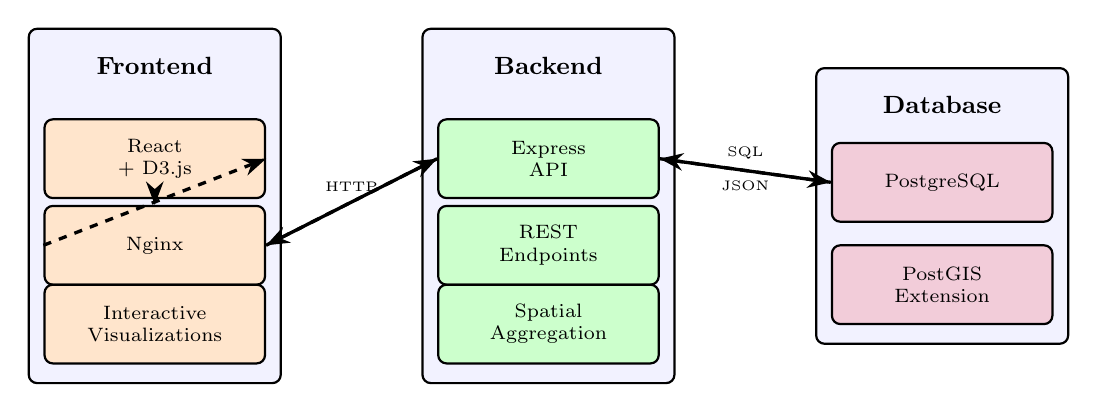
\begin{tikzpicture}[
        box/.style={rectangle, draw, thick, rounded corners=3pt, minimum height=1cm, minimum width=2.8cm, font=\scriptsize, align=center},
        container/.style={rectangle, draw, thick, rounded corners=3pt, minimum height=4.5cm, minimum width=3.2cm, fill=blue!5},
        arrow/.style={->, >=Stealth, very thick}
    ]
        % Frontend Container
        \node[container] (frontend_box) at (0,0) {};
        \node[font=\bfseries\small, anchor=north] at (frontend_box.north) [yshift=-0.25cm] {Frontend};
        \node[box, fill=orange!20] (react) at (0,0.6) {React\\+ D3.js};
        \node[box, fill=orange!20] (nginx) at (0,-0.5) {Nginx};
        \node[box, fill=orange!20] (viz) at (0,-1.5) {Interactive\\Visualizations};

        % Backend Container
        \node[container] (backend_box) at (5,0) {};
        \node[font=\bfseries\small, anchor=north] at (backend_box.north) [yshift=-0.25cm] {Backend};
        \node[box, fill=green!20] (express) at (5,0.6) {Express\\API};
        \node[box, fill=green!20] (endpoints) at (5,-0.5) {REST\\Endpoints};
        \node[box, fill=green!20] (aggregation) at (5,-1.5) {Spatial\\Aggregation};

        % Database Container
        \node[container, minimum height=3.5cm] (db_box) at (10,0) {};
        \node[font=\bfseries\small, anchor=north] at (db_box.north) [yshift=-0.25cm] {Database};
        \node[box, fill=purple!20] (postgres) at (10,0.3) {PostgreSQL};
        \node[box, fill=purple!20] (postgis) at (10,-1) {PostGIS\\Extension};

        % Arrows
        \draw[arrow] (react) -- (nginx);
        \draw[arrow] (nginx.east) -- (express.west) node[midway, above, font=\tiny] {HTTP};
        \draw[arrow] (express.east) -- (postgres.west) node[midway, above, font=\tiny] {SQL};
        \draw[arrow, dashed] (postgres.west) -- (express.east) node[midway, below, font=\tiny] {JSON};
        \draw[arrow, dashed] (express.west) -- (nginx.east);
        \draw[arrow, dashed] (nginx.west) -- (react.east);
    \end{tikzpicture}

    \vspace{0.5cm}
    \small
    Dockerized deployment with Nginx reverse proxy for API routing
\end{frame}

% ==============================================================================
\section{Visualization Techniques}
% ==============================================================================

\begin{frame}{Visualization 1: Spatial Heatmap}
    \centering
    \includegraphics[width=0.9\textwidth,height=0.8\textheight,keepaspectratio]{img/heatmap_placeholder.png}

    \vspace{5pt}
    \tiny{\textit{Spatial activity heatmap visualization}}
\end{frame}

\begin{frame}{Spatial Heatmap - Details}
    \textbf{Purpose}
    \begin{itemize}
        \item Visualize activity density across the city
        \item Identify busy areas and hotspots
        \item Track temporal patterns
    \end{itemize}

    \vspace{15pt}
    \textbf{Key Features}
    \begin{itemize}
        \item Grid-based aggregation
        \item Time slider (hourly/daily/weekly)
        \item Activity mode filtering
        \item Building polygon overlay
        \item Interactive zoom and pan
    \end{itemize}

    \vspace{15pt}
    \textbf{Technology}
    \begin{itemize}
        \item D3.js for rendering
        \item PostgreSQL spatial queries with PostGIS
    \end{itemize}
\end{frame}

\begin{frame}{Spatial Heatmap - Strengths}
    \textbf{Pros}
    \begin{itemize}
        \setlength{\itemsep}{10pt}
        \item Intuitive geographic representation
        \item Reveals spatial patterns at a glance
        \item Flexible temporal exploration
        \item Supports multiple aggregation levels
        \item Combines well with building overlays
        \item Effective for identifying hotspots
    \end{itemize}
\end{frame}

\begin{frame}{Spatial Heatmap - Limitations}
    \textbf{Cons}
    \begin{itemize}
        \setlength{\itemsep}{10pt}
        \item Grid resolution affects interpretation
        \item Can obscure individual movements
        \item Performance challenges with high granularity
        \item Requires spatial context to interpret
        \item May hide temporal variations within aggregates
    \end{itemize}
\end{frame}

\begin{frame}{Visualization 2: Activity Streamgraph}
    \centering
    \includegraphics[width=0.9\textwidth,height=0.8\textheight,keepaspectratio]{img/streamgraph_placeholder.png}

    \vspace{5pt}
    \tiny{\textit{Activity composition streamgraph over time}}
\end{frame}

\begin{frame}{Activity Streamgraph - Details}
    \textbf{Purpose}
    \begin{itemize}
        \item Show activity composition over time
        \item Reveal behavioral shifts
        \item Track participation trends
    \end{itemize}

    \vspace{15pt}
    \textbf{Key Features}
    \begin{itemize}
        \item Stacked area chart with smooth interpolation
        \item Multiple activity types (work, social, dining, etc.)
        \item Temporal filtering capabilities
        \item Color-coded activity categories
    \end{itemize}

    \vspace{15pt}
    \textbf{Key Insights Revealed}
    \begin{itemize}
        \item Work dominates weekdays
        \item Social activity peaks on weekends
        \item Meal times visible as distinct peaks
    \end{itemize}
\end{frame}

\begin{frame}{Activity Streamgraph - Strengths}
    \textbf{Pros}
    \begin{itemize}
        \setlength{\itemsep}{10pt}
        \item Shows composition and trends simultaneously
        \item Aesthetically appealing and engaging
        \item Reveals both macro and micro patterns
        \item Effective for time-series comparison
        \item Handles multiple categories elegantly
    \end{itemize}
\end{frame}

\begin{frame}{Activity Streamgraph - Limitations}
    \textbf{Cons}
    \begin{itemize}
        \setlength{\itemsep}{10pt}
        \item Difficult to read precise values
        \item Middle layers harder to interpret
        \item Can be overwhelming with too many categories
        \item Requires color differentiation
        \item Temporal aggregation may hide short-term spikes
    \end{itemize}
\end{frame}

\begin{frame}{Visualization 3: Activity Calendar}
    \centering
    \includegraphics[width=0.9\textwidth,height=0.8\textheight,keepaspectratio]{img/calendar_placeholder.png}

    \vspace{5pt}
    \tiny{\textit{Participant activity calendar (days $\times$ hours matrix)}}
\end{frame}

\begin{frame}{Activity Calendar - Details}
    \textbf{Purpose}
    \begin{itemize}
        \item Analyze individual daily routines
        \item Identify patterns and variations
        \item Compare participants side-by-side
    \end{itemize}

    \vspace{15pt}
    \textbf{Design}
    \begin{itemize}
        \item Days $\times$ Hours matrix
        \item Color-coded by activity type
        \item One month visible at a glance
        \item Scrollable timeline for full 15-month period
    \end{itemize}

    \vspace{15pt}
    \textbf{Use Cases}
    \begin{itemize}
        \item Find contrasting lifestyles
        \item Detect routine consistency
        \item Identify work schedules and patterns
    \end{itemize}
\end{frame}

\begin{frame}{Activity Calendar - Strengths}
    \textbf{Pros}
    \begin{itemize}
        \setlength{\itemsep}{10pt}
        \item Compact representation of long periods
        \item Patterns emerge naturally (work hours, weekends)
        \item Easy to spot anomalies and changes
        \item Effective for individual analysis
        \item Supports direct comparison
        \item Intuitive time-of-day interpretation
    \end{itemize}
\end{frame}

\begin{frame}{Activity Calendar - Limitations}
    \textbf{Cons}
    \begin{itemize}
        \setlength{\itemsep}{10pt}
        \item Limited to individual or small groups
        \item Requires significant screen space
        \item Can be cluttered with too many activity types
        \item Doesn't show spatial information
        \item Difficult to see population-level trends
    \end{itemize}
\end{frame}

\begin{frame}{Visualization 4: Building Polygons Overlay}
    \centering
    \includegraphics[width=0.9\textwidth,height=0.8\textheight,keepaspectratio]{img/buildings_placeholder.png}

    \vspace{5pt}
    \tiny{\textit{Building polygons overlaid on activity heatmap}}
\end{frame}

\begin{frame}{Building Polygons - Details}
    \textbf{Purpose}
    \begin{itemize}
        \item Provide spatial context for activity patterns
        \item Link activities to physical infrastructure
        \item Identify functional zones
    \end{itemize}

    \vspace{15pt}
    \textbf{Key Features}
    \begin{itemize}
        \item Filter by building type (residential, commercial, schools, etc.)
        \item Integrated with heatmap for layered context
        \item Color-coded by function
        \item Interactive toggle on/off
    \end{itemize}
\end{frame}

\begin{frame}{Building Polygons - Strengths}
    \textbf{Pros}
    \begin{itemize}
        \setlength{\itemsep}{10pt}
        \item Connects activity to infrastructure
        \item Helps explain spatial patterns
        \item Supports urban planning decisions
        \item Reveals functional zoning
        \item Combines well with other visualizations
    \end{itemize}
\end{frame}

\begin{frame}{Building Polygons - Limitations}
    \textbf{Cons}
    \begin{itemize}
        \setlength{\itemsep}{10pt}
        \item Can clutter the map
        \item Requires accurate building data
        \item May obscure underlying heatmap
        \item Static representation of dynamic spaces
    \end{itemize}
\end{frame}

\begin{frame}{Visualization 5: Participant Comparison}
    \centering
    \includegraphics[width=0.9\textwidth,height=0.8\textheight,keepaspectratio]{img/comparison_placeholder.png}

    \vspace{5pt}
    \tiny{\textit{Side-by-side participant comparison dashboard}}
\end{frame}

\begin{frame}{Participant Comparison - Details}
    \textbf{Purpose}
    \begin{itemize}
        \item Compare individual behavioral patterns
        \item Identify contrasting lifestyles
        \item Support hypothesis about proximity and well-being
    \end{itemize}

    \vspace{15pt}
    \textbf{Key Metrics}
    \begin{itemize}
        \item Daily travel distance
        \item Average joviality score
        \item Social activity percentage
        \item Work patterns
        \item Demographics
    \end{itemize}
\end{frame}

\begin{frame}{Participant Comparison - Strengths}
    \textbf{Pros}
    \begin{itemize}
        \setlength{\itemsep}{10pt}
        \item Direct quantitative comparison
        \item Reveals individual differences
        \item Supports finding extreme cases
        \item Evidence-based storytelling
        \item Helps answer "why" questions
    \end{itemize}
\end{frame}

\begin{frame}{Participant Comparison - Limitations}
    \textbf{Cons}
    \begin{itemize}
        \setlength{\itemsep}{10pt}
        \item Limited to 2-3 participants at once
        \item Doesn't show population distribution
        \item Risk of cherry-picking examples
        \item Requires manual selection
        \item No temporal dimension visible
    \end{itemize}
\end{frame}

\begin{frame}{Data Aggregation Strategy}
    \textbf{Spatial Aggregation}
    \begin{itemize}
        \item Grid-based binning (configurable cell size)
        \item \texttt{GROUP BY FLOOR(lat/cell\_size), FLOOR(lng/cell\_size)}
        \item Enables density calculation and hotspot identification
    \end{itemize}

    \vspace{8pt}
    \textbf{Temporal Aggregation}
    \begin{itemize}
        \item Hourly: Daily patterns and rush hours
        \item Daily/Weekly: Routine identification
        \item Monthly: Long-term trends
    \end{itemize}

    \vspace{8pt}
    \textbf{Activity Mode Filtering}
    \begin{itemize}
        \item Work, Home, Restaurant, Pub, Recreation, School, Shopping
        \item Supports focused analysis by activity type
        \item Reveals functional zones in the city
    \end{itemize}
\end{frame}

% ==============================================================================
\section{Key Findings}
% ==============================================================================

\begin{frame}{Question 1: City Areas - Overview}
    \textbf{Three Distinct Urban Zones Identified}

    \vspace{10pt}
    \begin{enumerate}
        \setlength{\itemsep}{15pt}
        \item \textbf{Downtown Commercial Core}
        \begin{itemize}
            \item Zones: B2, C2, C3
            \item High concentration of employers, restaurants, pubs
        \end{itemize}

        \item \textbf{Residential Zones}
        \begin{itemize}
            \item Zones: A1-2, B3-4, D2, D4
            \item Dominated by apartment buildings
        \end{itemize}

        \item \textbf{Mixed Suburban Areas}
        \begin{itemize}
            \item Zones: Northwest, Southeast
            \item Gradient from commercial to residential
        \end{itemize}
    \end{enumerate}

    \vspace{15pt}
    \textbf{Analysis Method:} Building type distribution, temporal activity patterns, movement flows
\end{frame}

\begin{frame}{Area 1: Downtown Commercial Core}
    \begin{columns}
        \begin{column}{0.5\textwidth}
            \textbf{Characteristics}
            \begin{itemize}
                \item High employer density
                \item Restaurants and pubs
                \item Peak activity: 9 AM - 6 PM
                \item Lower evening/night activity
            \end{itemize}

            \vspace{10pt}
            \textbf{Evidence}
            \begin{itemize}
                \item Building type concentration
                \item Business hours heatmap
                \item Commuter influx patterns
                \item Lunch hour spikes
            \end{itemize}
        \end{column}

        \begin{column}{0.45\textwidth}
            \centering
            \includegraphics[width=\textwidth,keepaspectratio]{img/q1_commercial_placeholder.png}

            \vspace{5pt}
            \tiny{\textit{Commercial building distribution}}

            \vspace{10pt}
            \includegraphics[width=\textwidth,keepaspectratio]{img/q1_business_hours_placeholder.png}

            \vspace{5pt}
            \tiny{\textit{Business hours activity}}
        \end{column}
    \end{columns}
\end{frame}

\begin{frame}{Area 2 \& 3: Residential and Mixed Zones}
    \begin{columns}
        \begin{column}{0.5\textwidth}
            \textbf{Residential Zones}
            \begin{itemize}
                \item High apartment concentration
                \item Peak: Evening/night
                \item Low daytime presence
                \item Social activity localized
            \end{itemize}

            \vspace{10pt}
            \textbf{Mixed Suburban}
            \begin{itemize}
                \item Commercial facing downtown
                \item Residential at periphery
                \item Limited connectivity (NW)
                \item Transitional character
            \end{itemize}
        \end{column}

        \begin{column}{0.45\textwidth}
            \centering
            \includegraphics[width=\textwidth,keepaspectratio]{img/q1_residential_placeholder.png}

            \vspace{5pt}
            \tiny{\textit{Residential building clusters}}

            \vspace{10pt}
            \includegraphics[width=\textwidth,keepaspectratio]{img/q1_evening_placeholder.png}

            \vspace{5pt}
            \tiny{\textit{Evening activity patterns}}
        \end{column}
    \end{columns}
\end{frame}

\begin{frame}{Question 2: Traffic Bottlenecks - Overview}
    \textbf{Three Critical Bottlenecks Identified}

    \vspace{15pt}
    \begin{enumerate}
        \setlength{\itemsep}{15pt}
        \item \textbf{Northwest Connector}
        \begin{itemize}
            \item MOST CRITICAL: Single route, no alternatives
            \item Severe rush hour congestion
        \end{itemize}

        \item \textbf{Downtown Corridors}
        \begin{itemize}
            \item Persistent through-traffic
            \item Multiple intersection points
        \end{itemize}

        \item \textbf{Southern Connector}
        \begin{itemize}
            \item Bidirectional bottleneck
            \item Residential convergence point
        \end{itemize}
    \end{enumerate}

    \vspace{15pt}
    \textbf{Rush Hour Patterns:} 7-9 AM (inbound) and 5-7 PM (outbound)
\end{frame}

\begin{frame}{Bottleneck Locations}
    \centering
    \begin{columns}
        \begin{column}{0.32\textwidth}
            \centering
            \includegraphics[width=\textwidth,height=0.6\textheight,keepaspectratio]{img/q2_northwest_placeholder.png}

            \vspace{3pt}
            \tiny{\textbf{Northwest bottleneck}}

            \tiny{Single-point failure}
        \end{column}
        \begin{column}{0.32\textwidth}
            \centering
            \includegraphics[width=\textwidth,height=0.6\textheight,keepaspectratio]{img/q2_center_placeholder.png}

            \vspace{3pt}
            \tiny{\textbf{Downtown congestion}}

            \tiny{Intersection clusters}
        \end{column}
        \begin{column}{0.32\textwidth}
            \centering
            \includegraphics[width=\textwidth,height=0.6\textheight,keepaspectratio]{img/q2_southeast_placeholder.png}

            \vspace{3pt}
            \tiny{\textbf{Southern connector}}

            \tiny{Residential convergence}
        \end{column}
    \end{columns}
\end{frame}

\begin{frame}{Temporal Traffic Patterns}
    \begin{columns}
        \begin{column}{0.48\textwidth}
            \centering
            \textbf{Morning Rush (7-9 AM)}

            \vspace{5pt}
            \includegraphics[width=\textwidth,height=0.55\textheight,keepaspectratio]{img/q2_morning_rush_placeholder.png}

            \vspace{5pt}
            \tiny{Residential $\rightarrow$ Commercial flow}
        \end{column}
        \begin{column}{0.48\textwidth}
            \centering
            \textbf{Weekend Pattern}

            \vspace{5pt}
            \includegraphics[width=\textwidth,height=0.55\textheight,keepaspectratio]{img/q2_weekend_placeholder.png}

            \vspace{5pt}
            \tiny{Uniform distribution, social clusters}
        \end{column}
    \end{columns}

    \vspace{10pt}
    \small
    \textbf{Key Insight:} Weekday bottlenecks disappear on weekends
\end{frame}

\begin{frame}{Question 3: Contrasting Lifestyles}
    \textbf{Selection Criteria}
    \begin{itemize}
        \item Used participant comparison tool
        \item Filtered by travel distance and joviality
        \item Found extreme opposites
    \end{itemize}

    \vspace{15pt}
    \begin{columns}
        \begin{column}{0.48\textwidth}
            \centering
            \textbf{Participant 266}

            \textbf{The Social Local}

            \vspace{10pt}
            \begin{tabular}{ll}
                Age: & 32 years \\
                Travel: & 5 units/day \\
                Joviality: & \textcolor{green}{\textbf{97.3\%}} \\
                Social: & 18.3\%
            \end{tabular}
        \end{column}

        \begin{column}{0.48\textwidth}
            \centering
            \textbf{Participant 845}

            \textbf{The Long Commuter}

            \vspace{10pt}
            \begin{tabular}{ll}
                Age: & 40 years \\
                Travel: & 32.2 units/day \\
                Joviality: & \textcolor{red}{\textbf{Below avg}} \\
                Social: & 5.2\%
            \end{tabular}
        \end{column}
    \end{columns}

    \vspace{15pt}
    \textbf{6× difference} in daily travel distance!
\end{frame}

\begin{frame}{Participant 266: The Social Local}
    \begin{columns}
        \begin{column}{0.5\textwidth}
            \textbf{Profile}
            \begin{itemize}
                \item Lives and works in city center
                \item Walking distance to work
                \item Avoids major bottlenecks
                \item Regular 9-5 schedule
            \end{itemize}

            \vspace{10pt}
            \textbf{Lifestyle}
            \begin{itemize}
                \item Frequent evening socializing
                \item Multiple social venues nearby
                \item Weekend social activities
                \item High quality of life
            \end{itemize}

            \vspace{10pt}
            \textbf{Impact}
            \begin{itemize}
                \item Very high joviality (97.3\%)
                \item Low time wasted commuting
                \item Strong social connections
            \end{itemize}
        \end{column}

        \begin{column}{0.45\textwidth}
            \centering
            \includegraphics[width=\textwidth,height=0.75\textheight,keepaspectratio]{img/q3_p266_placeholder.png}

            \vspace{3pt}
            \tiny{Regular work (orange), active social life (green)}
        \end{column}
    \end{columns}
\end{frame}

\begin{frame}{Participant 845: The Long Commuter}
    \begin{columns}
        \begin{column}{0.5\textwidth}
            \textbf{Profile}
            \begin{itemize}
                \item Home in south
                \item Work in east
                \item 2-hour daily commute
                \item Crosses multiple bottlenecks
            \end{itemize}

            \vspace{10pt}
            \textbf{Lifestyle}
            \begin{itemize}
                \item Leaves home at 7 AM
                \item Returns after 5 PM
                \item Limited evening time
                \item Minimal social activity
            \end{itemize}

            \vspace{10pt}
            \textbf{Impact}
            \begin{itemize}
                \item Below-average joviality
                \item High time burden
                \item Reduced life satisfaction
            \end{itemize}
        \end{column}

        \begin{column}{0.45\textwidth}
            \centering
            \includegraphics[width=\textwidth,height=0.75\textheight,keepaspectratio]{img/q3_p845_placeholder.png}

            \vspace{3pt}
            \tiny{Long commutes (red), limited social time}
        \end{column}
    \end{columns}
\end{frame}

\begin{frame}{Key Insight: Proximity Matters}
    \centering
    \includegraphics[width=0.85\textwidth,height=0.6\textheight,keepaspectratio]{img/q3_comparison_placeholder.png}

    \vspace{10pt}
    \Large
    \textbf{Geographic proximity between home, work,}

    \textbf{and amenities profoundly impacts}

    \textbf{quality of life and well-being}

    \vspace{10pt}
    \normalsize
    Urban planning should prioritize reducing commute distances
\end{frame}

\begin{frame}{Question 4: Temporal Changes (1/2)}
    \textbf{Major Trends Over 15 Months}

    \vspace{10pt}
    \begin{enumerate}
        \setlength{\itemsep}{10pt}
        \item \textbf{Initial Adjustment Period} (Days 1-60)
        \begin{itemize}
            \item Elevated activity in first weeks → normalization
        \end{itemize}

        \item \textbf{Early Social Surge}
        \begin{itemize}
            \item High social engagement weeks 1-4
            \item Transition to sustainable routines
        \end{itemize}

        \item \textbf{Activity Composition Stability}
        \begin{itemize}
            \item Despite participant dropout, proportions stable
            \item Work dominates weekdays, social on weekends
        \end{itemize}

        \item \textbf{Weekend vs Weekday Transformation}
        \begin{itemize}
            \item Weekday: Employment travel
            \item Weekend: Social/dining journeys
        \end{itemize}

        \item \textbf{Individual Persistence}
        \begin{itemize}
            \item Personal "behavioral fingerprints" stable
            \item Routines consistent across 15 months
        \end{itemize}
    \end{enumerate}
\end{frame}

\begin{frame}{Question 4: Temporal Changes (2/2)}
    \begin{enumerate}
        \setlength{\itemsep}{10pt}
        \setcounter{enumi}{5}
        \item \textbf{Spatial Clustering Evolution}
        \begin{itemize}
            \item Dispersion → concentration over time
            \item Participants find preferred venues
        \end{itemize}

        \item \textbf{Venue Popularity Cycles}
        \begin{itemize}
            \item "Flash popularity": 2-4 week surges
            \item Some permanent, some temporary hotspots
        \end{itemize}

        \item \textbf{Multi-Activity Evenings}
        \begin{itemize}
            \item 18:00-21:00: 5-6 activity types simultaneously
            \item Mornings: Work dominates
        \end{itemize}

        \item \textbf{Interest Group Homogeneity}
        \begin{itemize}
            \item Minimal demographic divergence
            \item Spatial constraints override demographics
        \end{itemize}

        \item \textbf{Cyclical Variations}
        \begin{itemize}
            \item Seasonal/circumstantial influences
            \item Recurring social/dining patterns
        \end{itemize}
    \end{enumerate}
\end{frame}

\begin{frame}{Temporal Evolution Evidence}
    \begin{columns}
        \begin{column}{0.48\textwidth}
            \centering
            \textbf{15-Month Overview}

            \vspace{5pt}
            \includegraphics[width=\textwidth,height=0.55\textheight,keepaspectratio]{img/q4_evolution_placeholder.png}

            \vspace{3pt}
            \tiny{Participant dropout, stable activity proportions}
        \end{column}
        \begin{column}{0.48\textwidth}
            \centering
            \textbf{Daily Patterns}

            \vspace{5pt}
            \includegraphics[width=\textwidth,height=0.55\textheight,keepaspectratio]{img/q4_daily_placeholder.png}

            \vspace{3pt}
            \tiny{Work, social, eating rhythms}
        \end{column}
    \end{columns}

    \vspace{10pt}
    \small
    \textbf{Observation:} Macro-level changes coexist with micro-level stability
\end{frame}

% ==============================================================================
\section{Recommendations}
% ==============================================================================

\begin{frame}{Key Insights Summary}
    \Large
    \begin{enumerate}
        \setlength{\itemsep}{20pt}
        \item \textbf{Spatial:} Clear functional zones, northwest vulnerable

        \item \textbf{Traffic:} Predictable rush hour bottlenecks

        \item \textbf{Behavioral:} Proximity correlates with well-being

        \item \textbf{Temporal:} Individual stability, population dynamics
    \end{enumerate}
\end{frame}

\begin{frame}{Urban Planning Recommendations}
    \textbf{Priority 1: Infrastructure}
    \begin{itemize}
        \item Create alternative route to northwest zone
        \item Expand downtown corridor capacity
        \item Implement traffic management systems
    \end{itemize}

    \vspace{15pt}
    \textbf{Priority 2: Development}
    \begin{itemize}
        \item Promote mixed-use development
        \item Reduce residential-workplace distances
        \item Support local social venues
    \end{itemize}

    \vspace{15pt}
    \textbf{Priority 3: Quality of Life}
    \begin{itemize}
        \item Design for walkability
        \item Plan around behavioral patterns, not just demographics
        \item Enable 15-minute neighborhoods
    \end{itemize}
\end{frame}

% ==============================================================================
\section{Reflection}
% ==============================================================================

\begin{frame}{Strengths \& Limitations}
    \begin{columns}
        \begin{column}{0.48\textwidth}
            \textbf{Strengths}
            \begin{itemize}
                \item Interactive exploration
                \item Multi-scale analysis
                \item Evidence-based insights
                \item Scalable architecture
                \item Accessible visualizations
            \end{itemize}

            \vspace{10pt}
            \textbf{Future Enhancements}
            \begin{itemize}
                \item Flow diagrams
                \item Speed heatmaps
                \item Predictive modeling
                \item Real-time integration
            \end{itemize}
        \end{column}

        \begin{column}{0.48\textwidth}
            \textbf{Limitations}
            \begin{itemize}
                \item Sample representativeness
                \item No causal analysis
                \item Performance constraints
                \item Learning curve
            \end{itemize}

            \vspace{10pt}
            \textbf{Applicability}
            \begin{itemize}
                \item Urban planning
                \item Transportation analysis
                \item Behavioral studies
                \item Decision support
            \end{itemize}
        \end{column}
    \end{columns}
\end{frame}

\begin{frame}{Key Takeaways}
    \Large
    \begin{enumerate}
        \setlength{\itemsep}{20pt}
        \item \textbf{PostGIS essential} for spatial data

        \item \textbf{Iterative design} reveals insights

        \item \textbf{Performance matters} for 18GB datasets

        \item \textbf{Context drives interpretation}

        \item \textbf{Visual analytics} enables discovery
    \end{enumerate}
\end{frame}

% ==============================================================================
\section{Conclusion}
% ==============================================================================

\begin{frame}{Summary: Challenge Accomplished}
    \Large
    \textbf{Answered All Four Questions}

    \vspace{15pt}
    \normalsize
    \begin{enumerate}
        \setlength{\itemsep}{12pt}
        \item \textbf{City Areas:} 3 distinct zones identified

        \item \textbf{Bottlenecks:} 3 critical congestion points

        \item \textbf{Routines:} 6× difference in commute impacts life

        \item \textbf{Changes:} 10 temporal patterns documented
    \end{enumerate}

    \vspace{20pt}
    \Large
    \textbf{Delivered actionable urban planning insights}

    \textbf{through interactive visual analytics}
\end{frame}

\begin{frame}{}
    \centering
    \vspace{2cm}
    {\Huge \textbf{Thank You!}}

    \vspace{1.5cm}
    {\large Questions?}

    \vspace{1.5cm}
    \begin{tabular}{ccc}
        Alberto Finardi & Tommaso Crippa & Tom Gave \\
    \end{tabular}

    \vspace{0.8cm}
    \scriptsize
    Data Visualization -- University of Luxembourg

    \vspace{0.5cm}
    {\tiny VAST Challenge 2022: Challenge 2 - Patterns of Life}
\end{frame}

\end{document}
